\documentclass{article}

\usepackage{comment}
\usepackage{graphicx}
\usepackage{hyperref} 
\usepackage{geometry}

\geometry{margin=1cm}

\newcommand{\labelCaption}[2] {\vspace{.25in} \hrule\vspace{0.5em}
\noindent{\bf #1: #2} \vspace{0.5em}
\hrule \vspace{.10in}}

\newcommand{\explanation}[2] {\vspace{.25in} \hrule\vspace{0.5em}
\noindent{\bf #1} \vspace{0.5em}
\hrule \vspace{.10in}}

\begin{document}

\begin{center}
  {\Large Gender Studies\ Final} \\
  Adele Swecker
\end{center}

\labelCaption{To access the code and pictures for this project you can go to the following link}

{\Large
  \href{https://github.com/als471/Gender-Studies-Final-Project}{Github Repository}}

%  You will be asked to provide a description of approximately 300-500 words 
% talk about your creation, why you chose to create it, and how it reflects your engagement with the class.

\explanation{\ \ \ For my final project, I decided to transform our readings into readable PDF files. I did this so that I can 
process each PDF to analyze and extract information from our assigned materials. I decided to focus on 
recognizing important keywords and their prevalence in our texts to highlight the bias present in said texts. 
I developed a computer program capable of reading through each document, parsing by word and then tallying the 
occurrences of each specific word. After finishing the tally, I decided on a list of words that I believed showcase 
the bias present in our readings. After outputting the tally, I inputted the counts into a program that would output the graphs
that are showed below.\\

I decided to create this program as a way to identify and analyze reoccurring words and themes present in our readings. 
I compiled a short list of words to focus on to highlight this: "her," "him," "woman," "man," "white," "black," "race," 
"gender," "sex," and "sexual." I attempted to shed light on any underlying patterns of occurrence of feminine words vs masculine words 
and any racial bias as well. These terms were selected because I believe they present a balance of gender and racial phrases that 
will accurately portray the bias I'm hoping to showcase.\\

After running my program and generating the word counts, I was able to internalize my findings. 
One notable observation was the differences in gender-specific pronouns and adjectives. The female pronouns and 
adjectives such as "her" and "woman" consistently appeared twice as often as their male counterparts, "him" and 
"man." This discovery showcased the representation of gender within our readings and showcases the bias in our 
readings. Obviously, as a gender and science class, it makes sense that we would hear more about female's in our readings 
than males but I still thought that the direct bias in readings was interesting to portray in the graphs below.}

\break

\labelCaption{To visually represent my findings, I created a graph to showcase the word counts of the chosen words as well as a control
  word in "the". Because of the prevalence with which the word "the" shows up in most writings, I believed that it would showcase 
  the frequency with which other words are appearing. This graph is meant to visualize the word counts and biases in a way that 
  is readable and understandable}

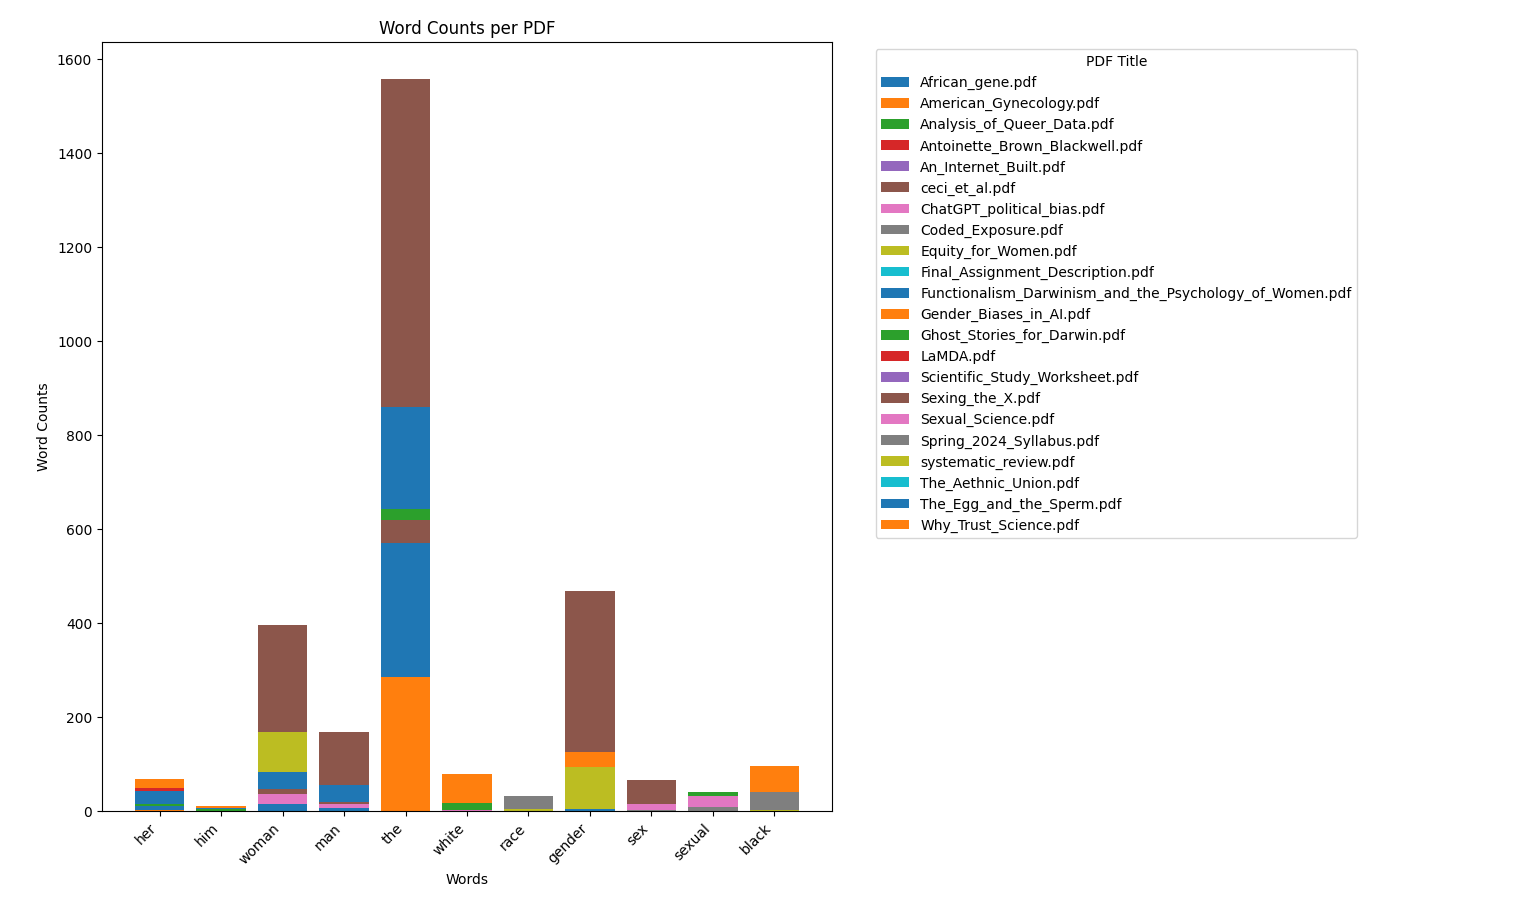
\includegraphics[width=\textwidth]{word counts including the.png}

\break

\labelCaption{The other graph I decided to showcase, was one without our control word as I wanted the inherit bias to be able to speak for 
itself and i believed it was important for you to be able to see the comparisons in word counts without the distraction of our control 
word count}

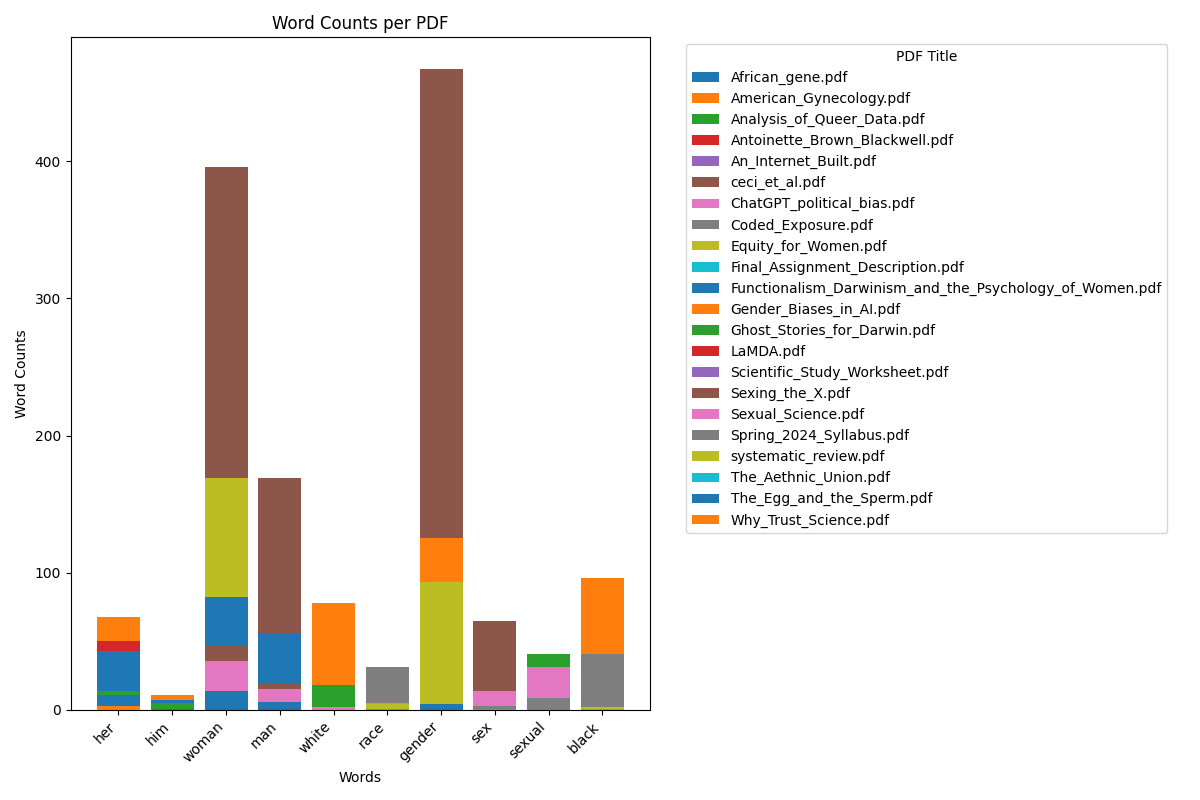
\includegraphics[width=\textwidth]{word counts.png}

\explanation{Overall, my project showcases my engagement with this class because I thought of this idea during our classes where we were 
looking at the bias in recommendation letters as well as bias in the science field as a whole. Through the development of my 
computer program, I hoped to shed light onto the bias in the readings in our class. I also very much enjoyed writing this program as 
I will be able to reused it for other purposes and in other classes}


\end{document}